\documentclass[12pt,a4paper]{book}
\usepackage[T1]{fontenc}
\usepackage[utf8]{inputenc}
\usepackage[portuguese]{babel}
\usepackage{hyperref}
\usepackage{graphicx}
\usepackage{amsmath,amssymb,amsthm}
%\usepackage{tikz}
%\usepackage{thmtools}
\usepackage{proof}
\usepackage{pifont,comment}
\usepackage{listingsutf8}
\usepackage{color}
%\usepackage{algorithm}
%\usepackage{multirow}
%\usepackage{etoolbox}
%\usepackage{epigraph}

%\usepackage[latin1]{inputenc}

%\usetikzlibrary{trees}

%% dedication environment

\newenvironment{dedication}
{
   \cleardoublepage
   \thispagestyle{empty}
   \vspace*{\stretch{1}}
   \hfill\begin{minipage}[t]{0.66\textwidth}
   \raggedright
}
{
   \end{minipage}
   \vspace*{\stretch{3}}
   \clearpage
}

\makeatletter
\renewcommand{\@chapapp}{}% Not necessary...
\newenvironment{chapquote}[2][2em]
  {\setlength{\@tempdima}{#1}%
   \def\chapquote@author{#2}%
   \parshape 1 \@tempdima \dimexpr\textwidth-2\@tempdima\relax%
   \itshape}
  {\par\normalfont\hfill--\ \chapquote@author\hspace*{\@tempdima}\par\bigskip}


\graphicspath{{figuras/}{../figuras/}{../../figuras/}}
%\graphicspath{{subdir1/}{subdir2/}{subdir3/}...{subdirn/}}

\newcommand{\minizinc}{MiniZinc}
\newcommand{\PR}{Programação por Restrições}


\textwidth=16.4cm 
\textheight=22cm

\headsep = 0.5cm
\topmargin=-0.5cm 

\oddsidemargin = -0.30cm 
\evensidemargin= -0.30cm 


\makeatother


% Book's title and subtitle
\title{\Huge \textbf{Modelos Computacionais com Programação por Restrições}}
% Author
\author{\textsc{Claudio Cesar de Sá e outros}}


\begin{document}

\definecolor{mygreen}{rgb}{0,0.6,0}
\definecolor{mygray}{rgb}{0.5,0.5,0.5}
\definecolor{mymauve}{rgb}{0.58,0,0.82}

\lstset{ %
  backgroundcolor=\color{white},   % choose the background color; you must add \usepackage{color} or \usepackage{xcolor}
  basicstyle=\normalsize\ttfamily,        % the size of the fonts that are used for the code
  breakatwhitespace=false,         % sets if automatic breaks should only happen at whitespace
  breaklines=true,                 % sets automatic line breaking
  captionpos=b,                    % sets the caption-position to bottom
  commentstyle=\color{mygreen},    % comment style
  deletekeywords={},               % if you want to delete keywords from the given language
  escapeinside={\%*}{*)},          % if you want to add LaTeX within your code
  extendedchars=true,              % lets you use non-ASCII characters; for 8-bits encodings only, does not work with UTF-8
  frame=none,                    % adds a frame around the code
  keepspaces=true,                 % keeps spaces in text, useful for keeping indentation of code (possibly needs columns=flexible)
  keywordstyle=\color{red},       % keyword style
  language=Octave,                 % the language of the code
  morekeywords={*,Inductive, Set, Definition, Fixpoint,match,with}, % if you want to add more keywords to the set
  numbers=none,                    % where to put the line-numbers; possible values are (none, left, right)
  numbersep=5pt,                   % how far the line-numbers are from the code
  numberstyle=\tiny\color{mygray}, % the style that is used for the line-numbers
  rulecolor=\color{black},         % if not set, the frame-color may be changed on line-breaks within not-black text (e.g. comments (green here))
  showspaces=false,                % show spaces everywhere adding particular underscores; it overrides 'showstringspaces'
  showstringspaces=false,          % underline spaces within strings only
  showtabs=false,                  % show tabs within strings adding particular underscores
  stepnumber=2,                    % the step between two line-numbers. If it's 1, each line will be numbered
  stringstyle=\color{mymauve},     % string literal style
  tabsize=2,                       % sets default tabsize to 2 spaces
  title=\lstname ,                 % show the filename of files included with \lstinputlisting; also try caption instead of title
  identifierstyle={\normalsize\ttfamily\color{blue}}
}

\frontmatter
\maketitle

\tableofcontents
%\listoffigures
%\listoftables

\mainmatter

%\input{meta-keys}


\chapter*{Nota desta Versão Experimental}


\section*{Autores}

Este é um livro experimental (projeto de uma publicação a longo prazo) e tem muitos autores. Dentre eles cita-se:

\begin{enumerate}
\item Marcos Creuz Filho
\item Lucas Hermman Negri
\item ..........
\item Ajudando ... reservado para incluirmos o seu nome  ...

\end{enumerate}


\section*{Sobre o Livro}

\begin{enumerate}
\item Este livro tem um foco: é o título do livro. Alguns modelos
clássicos de problemas, alguns originais, 
são discutidos, modelados e implementados em Minizinc.

\item O Minizinc foi escolhido pela sua leitura próxima a formulação
matemática. Voce irá gostar desta linguagem orientada a modelos;


\item Este livro, parte dele, é resultado de alguns semestres de ensino de graduação no curso de Ciência da Computaçao da UDESC, de uma disciplina optativa introdutória
a Programação por Restrições (PR).

%\item 

\end{enumerate}


\section*{Resumindo ....}

A proposta deste livro é completamente {\bf \textcolor{red}{embrionária}}.  Neste primeiro
momento, há um {\em copy-paste} de um TCC aqui da UDESC--Joinville, que orientei. Contudo, há  muito material escrito
que falta organizar dentro desta proposta.

Assim, vá me cobrando por email, \url{claudio.sa@udesc.br},
que vou aprontando o material na medida que as perguntas surgerirem.


%\part{L\'ogica Formal}

\chapter{Complexidade de Problemas}
\label{cp:complexidade}


Neste capítulo são apresentados os fundamentos sobre
complexidade de problemas.  Avaliar o que são problemas
exponenciais e o quanto são complexos.



\section{Mapeando o Territ\'orio}


Os problemas combinatoriais são ubíquos no cotidiano de pessoas, indústria, etc.
Basicamente utiliza-se alguma estimativa entre combinar objetos,
pessoas versus recursos para se atingir algum objetivo.
Em termos matemáticos, tem-se variáveis tais como $x_1$, $x_2$, $x_3$, etc, a terem
seus valores instanciados sobre algum domínio ou terem alguma relação
com outras variáveis, segundo algum critério ou requisito.

Exemplificando, voce quer organizar um calendário de jogos para os times da
sétima divisão de sua cidade. Assim, os $n$ times devem fazer um rodízio
nos $2$ campos disponíveis, tal que todo sábado  tenham $2$ jogos
por campo. Logo, serão $8$ times jogando num final de semana. Basicamente
voce deve distribuir estes encontros entre dois times respeitando critérios
como:
\begin{enumerate}
\item Local do jogo: todos os times devem jogar igualmente nos dois campos.
Afinal, um deles tem grama e a bola \textit{corre redonda};
\item Espaçamento entre os encontros: os times devem jogar até o final
da temporada;
\item Devem alternar o horário de jogo: afinal, se seu time tiver o primeiro
jogo da tarde, a feijoada está comprometida.
\end{enumerate}

Enfim, este simples ensaio mostra o cotidiano de situações combinatoriais
em que tudo se apresenta. Estes problemas vem sendo atacados há séculos tendo 
Euler como um dos matemáticos precursores, ao analisar o problema das 7 pontes 
das  Königsberg. A representação por meio de grafos foi uma estratégia
de analisar e solucionar o problema. O problema do caminho euleriano é
 base de vários estudos, pois sua  tratabilidade o coloca na classe
 de problemas NP \cite{sipser12}.

Neste encaminhamento, várias áreas de pesquisa  estão focadas como: Pesquisa
Operacional, Computação Evolutiva, Inteligência Artificial (IA), Programação por
Restrições (PR), etc. O contexto desta pesquisa encontra-se dentro destas duas 
últimas áreas, mais especificamente a \PR .


\subsection{Problemas em Inteligência Artificial}

Diversas áreas estão associadas à Inteligência Artificial como tradução de línguas, interpretação de regras, robótica em geral,  manipulação de dados em imagens,
 planejamento, reconhecimento  e outras atividades. Uma das caraterísticas destes problemas 
é a sua complexidade algoritmica e computacional, que em geral crescem exponencialmente.
Dado este fato, há uma dificuldade inerente na tarefa do desenvolvimento de algoritmos
 e solucoes aceitáveis. Estes aspectos se relacionam a área de tratabilidade de problemas,
 os quais delineam as fronteiras dos limites dos problemas em aceitarem
 soluções em um tempo razoáveis de processamento.


Para encontrar uma solução  aos problemas abordados pela IA é necessário que o processo de análise seja detalhado e modelado de 
acordo com técnicas específicas. Neste sentido duas áreas da IA são destacadas \cite{RusNorv2010}: \textit{representação do 
conhecimento}  e aplicação de \textit{métodos de busca}. Estas duas áreas apresentam uma interseção a \PR  pois os problemas quando 
atacados com PR necessitam apresentar um \textit{modelo} a ser computado e esquemas
de buscas sobre os espaço de estados que o mesmo exibe. Um dos  resultados
de uma solução com PR é a construção deste modelo, sob o qual as restrições serão
postadas, e avaliadas segundo um mecanismo \textit{completo} de busca.
 Em PR o tema da modelagem 
é investigado em \cite{smith_2006} e buscas em \cite{beek_2006,hoos_2006}.

%%% There are three main algorithmic techniques for solving constraint satisfaction problems:
%%% backtracking search, local search, and dynamic programming. 

%%% MR Jones, Patinoeire, clermont, 17:21, 24/out

\subsection{Problemas de Satisfação de Restrições}
\label{sec:ch_cp}

Um problema combinatorial cl\'assico é apresentado por um conjunto de vari\'aveis de um sistema,  as quais  ser\~ao instanciadas por objetos de domínios, segundo um conjunto de relaç\~oes, as quais representam o relacionamento entre os objetos. A tarefa combinatorial
é dada pela aç\~ao de instanciar estes objetos as variáveis, de tal modo que todas as 
relaç\~oes sejam satisfeitas.

A esta classe de problemas combinatoriais é conhecida como \textit{Problemas de Satisfação de Restrições} (PSRs). A resoluç\~ao dos PSR's constituem em encontrar valores as variáveis
respeitando ou satisfazendo suas restrições. Para esta classe de problemas lança-se mão do uso da \textit{Programação por Restrições} (PPR ou PR), ou seja, uma técnica que utiliza uma teoria e  ferramentas pr\'oprias de  programação. A PPR é uma forma de aplicar os conceitos de variáveis, domínios e restrições, via esta teoria específica de programação. 

Um PSR é tipicamente um problema \textit{NP-Completo} \cite{rossi_2006}. O desafio de todo o processamento por restrições está em gerar algoritmos que resolvam esta classe de problemas em um tempo
computacional aceitável. Invariavelmente, alguns destes problemas NP, podem apresentar uma
complexidade espacial consider\'avel, assim passam para classe P-SPACE \cite{sipser12}.
Dado este aspecto combinatorial e de complexidade NP, esta passa ter interesse
por outras àreas da pesquisa que lidam buscas \textit{heurísticas}, tais como a Computação Evolutiva (CE),
 ou ainda buscas \textit{completas} com a IA clássica e a Pesquisa Operacional (PO), etc. Esta situaçao é ilustrada pela figura \ref{fig:eureka}.


\begin{figure}[!ht]
\begin{center}
%%%  \includegraphics[scale=0.5]{figuras/psr_01.eps}
  \caption{Família dos problemas do tipo satisfação de restrições}
\label{fig:eureka}
\end{center}
\end{figure}


A \PR por sua vez, a exemplo da IA, CE, PO, etc, apresenta várias outras
subdivisões e sub-áreas de interesse.  Uma delas ela é a \textit{Programação em Lógica com Restrições} (PLR) um dos segmentos a serem atacados nesta pesquisa. A PLR tem na lógica de primeira-ordem 
o seu modelo computacional, o qual é calculado a partir de buscas exaustivas sobre
os seus \textit{modelos consistentes} (modelos de Herbrand).

Uma das   partes mais instigantes sobre os PSRs é que os mesmo são onipresentes
em problemas do mundo real. Alguns destes  problemas são discutidos em \cite{rossi_2006}.
Destancam-se os problemas de escalonamento, planejamento, roteamento, contenção,
alocação, etc.

As restrições podem ser consideradas como informações e dados há um programa por restrições. 
Estas  visam limitar o \textit{espaço de busca} e descrevem propriedades de 
variáveis/objetos e o relacionamento entre eles. As restrições são formalizadas como uma relação entre os objetos e esses são modelados como variáveis \cite{fruewirth2003}.

A relação existente entre os problemas de satisfação de restrições e a programação por restrições é expressa pela figura \ref{fig:eureka}. Portanto, pode-se considerar que a PR está contida em PSR. Ou seja, a PR é um método que pode ser aplicado para encontrar a solução de problemas do tipo PSR.

Na PR, se a abordagem for feita via programação em lógica, então tem-se a PLR. A PLR é atrativa sob os seguintes requisitos metodológicos:

\begin{itemize}
\item Adequação a representação do conhecimento, caso este seja construído em lógica formal;
\item Rápida prototipação e consequentemente baixo custo de desenvolvimento;
\item Visão declarativa de suas restrições, possibilitando uma facilidade quanto aos testes e depuração;
\item Flexibilidade na codificação dos algoritmos por abstrair características de programação em lógica.
\end{itemize}

Contudo, a Programação em Lógica com Restrições é resultado da utilização do paradigma da programação em lógica somado à programação por restrições. A PLR está contida no subconjunto de técnicas que fazem uso da PL para resolver problemas do tipo PSR. As vantagens de se utilizar a programação em lógica por restrições (PLR) estão em: modelar problemas de forma declarativa com uma sólida base matemática, propagação dos efeitos das decisões utilizando algoritmos eficientes e busca por soluções ótimas \cite{fruewirth2003}. Desde o início dos anos 90, a programação baseada em restrições tem tido sucesso comercial e industrial \cite{RusNorv2010}. Em 1996, o mundo gerou, utilizando tecnologia de restrições um valor estimado de 100 milhões de dólares \cite{fruewirth2003}.


\textcolor{red}{refazer as secoes anteriores}


\section{Complexidade}


\textcolor{red}{Refazer o Conteudo anterior e acrescentar o tema sobre complexidade e problemas P e NP e com isto o que a PR resolve}

\section{Árvores de Buscas: Ilustrando a Complexidade}

\textcolor{red}{acrescentar conteúdo dos slides do curso ... }



\section{Conclusões Parciais}
{\bf \textcolor{red}{Faltando .... e melhorar a apresentacao acima}}

\chapter{Programação por Restrições}\label{cp:pr}


Este capítulo visa prover uma base de como a PR funciona.


\section{Apresentando a PR}

A Programação por Restrições (PR) é um paradigma de programação, tal como o paradigma imperativo, o orientado a objetos, o funcional, o lógico e outros. A idéia geral da PR, conforme \cite{thom}, é de resolver problemas simplesmente declarando restrições que devem ser satisfeitas pelas soluções destes.

De acordo com \cite{apt}, a PR já foi aplicada com sucesso em diversas áreas, como biologia molecular, engenharia elétrica, pesquisa operacional e análise numérica. Entre as principais aplicações, pode-se citar sistemas de suporte à decisão para problemas de escalonamento e alocação de recursos \cite{thom}.

Problemas que hoje são identificados como sendo de satisfação de restrições, como por exemplo programar os horários de trabalho em uma empresa, sempre estiveram naturalmente presentes de alguma forma com a humanidade. Entretanto, métodos específicos para solucionar este tipo de problema começaram a surgir no meio acadêmico apenas nas décadas de 1950 e 1960, apesar de que técnicas como o \textit{backtracking} (um método de busca exaustiva refinado) já eram utilizadas de forma recreativa desde o século XIX \cite{cphandbook}.

A Seção \ref{sc-conceitos-basicos-pr} apresenta alguns conceitos básicos deste paradigma, de forma a esclarecer como este funciona e o que o difere do paradigma imperativo. A Seção \ref{sc-modelagem} esclarece as propriedades da modelagem de problemas por meio de uma linguagem de PR. A Seção \ref{sc:minizinc} apresenta a linguagem MiniZinc e demonstra alguns recursos da linguagem com o auxílio de um exemplo.



\section{Ilustrando os Conceitos}
\label{sc-conceitos-basicos-pr}

Algumas definições de termos comumente utilizados na área são apresentadas em \cite{leler}. Conforme este, uma restrição expressa uma relação desejada entre um ou mais objetos. Uma linguagem de PR é uma linguagem que possibilita descrever os objetos e as restrições. Um programa feito em uma linguagem de PR define um conjunto de objetos e um conjunto de restrições sobre estes objetos. Um sistema de satisfação de restrições encontra soluções para programas feitos em uma linguagem de PR, ou seja, atribui valores aos objetos de forma que todas as restrições sejam satisfeitas.

Conforme \cite{stuckey}, as restrições presentes no mundo real podem ser modeladas por meio de restrições em linguagem matemática. Desta forma, os objetos que tais restrições relacionam são também de cunho matemático, tais como variáveis e números.

Um exemplo simples apresentado em \cite{leler} é a conversão de temperaturas. Por exemplo, a restrição:
\[
  C = (F - 32) \times \frac{5}{9}
\]
define o relacionamento entre temperaturas em Fahrenheit e Celsius, representadas respectivamente pelas variáveis $C$ e $F$.

Em \cite{leler}, também é reforçado o fato de que o sinal de igualdade em linguagens de PR possui o mesmo sentido da igualdade matemática. Isto difere-se de grande parte das linguagens imperativas (por exemplo C, Java e Python), nas quais o sinal de igualdade representa a operação de atribuir um valor a uma variável. Desta forma, em uma linguagem de PR, a restrição acima poderia ser reescrita, por exemplo, da seguinte forma:
\[
  9 \times C = 5 \times (F - 32)
\]

Como tal restrição descreve o relacionamento entre as variáveis $C$ e $F$, a partir do momento em que uma das variáveis receber um valor, o valor da outra variável já pode ser calculado. Além disto, caso fosse necessário realizar conversões para a escala Kelvin, bastaria adicionar a seguinte restrição:
\[
  K = C - 273
\]

em que $K$ é a variável que representa a temperatura em Kelvin. Assim como na restrição anterior, caso o valor de uma das variáveis for conhecido, o valor da outra pode ser calculado. Além disto, as restrições pertencentes ao conjunto de restrições de um dado programa são dependentes entre si. Desta forma, apenas com estas duas restrições é possível converter temperaturas entre Kelvin e Fahrenheit, sem explicitar a fórmula de conversão entre tais unidades \cite{leler}.

Entretanto, as restrições não se limitam à equações lineares. Os tipos de restrição e de domínios de variáveis variam dependendo da linguagem. Os tipos comuns de domínio de variáveis são, por exemplo, inteiros, reais, booleanos, conjuntos, vetores, e outros. Também se faz possível declarar inequações, por exemplo, por meio dos operadores $\ge$ e $\not=$.

As operações possíveis entre as variáveis também variam, mas normalmente se faz possível utilizar as operações aritméticas básicas, como $+, -, /, \times$, para inteiros e reais, operadores lógicos, como $\wedge, \vee, \rightarrow, \leftrightarrow$, para booleanos, operações como $\cup$ e $\cap$ para conjuntos, entre outros.

Outro tipo de domínio de grande importância para a PR são os domínios finitos. Os valores possíveis que uma variável de domínio finito pode receber são restritos a um conjunto finito de valores. Um exemplo clássico de domínio finito é o domínio booleano, no qual as variáveis só podem receber os valores \textit{true} ou \textit{false}. Outro exemplo são os intervalos de valores inteiros, como $[1,10]$, por exemplo.

Os domínios finitos são amplamente utilizados na PR por permitirem ao programador modelar de forma natural problemas que envolvem escolhas, representando cada uma das possíveis escolhas por meio dos valores presentes no domínio \cite{stuckey}.



 \section{Elementos ou Formalizando a  PR}

Esta seção é   didaticamente apresentada por alguns fundamentos da PR, pois, estes elementos
se descrevem as restrições  e declarações sob um problema. Os problemas devem ser modelados, categorizados, ou seja, representados de forma a fazer com que se possa aplicar um determinado método de busca para encontrar a(s) solução(ões). Diversas são as técnicas encontradas na IA para a modelagem e resolução de problemas \cite{RusNorv2010}.

Uma delas é a aplicação de técnicas para a solução de Problemas de Satisfação de Restrições - PSR, ou, problemas que podem ser resolvidos pelo uso de restrições.

Um problema de satisfação de restrições (PSR) é uma tupla $(V,D,R)$ onde \cite{apt_2003}:

\begin{itemize}

 \item $V$ é um conjunto de $n$ variáveis $\lbrace x_{1}, ..., x_{n} \rbrace$. Por convenção, variáveis  são representadas pelas letras $x$, $y$, $z$, etc, indexadas por $i$ se for caso de um número
 significativo das mesmas; fato que é regra geral.
 

 \item $D = \lbrace D_{1}, ..., D_{n} \rbrace$ é um conjunto de domínios. Onde cada componente $D_{i}$ é o domínio que contém todos os possíveis valores que se podem atribuir à variável $x_{i}$.


 \item $R$ é um conjunto finito de restrições. Cada restrição $n$-ária $(R_{n})$ está definida sobre um conjunto de variáveis $\lbrace x_{1}, ..., x_{x} \rbrace$ restringindo os valores que as variáveis podem, simultaneamente possuir. Este conjunto é dado por: $R = \{ r_1, r_2, ..., r_m \}$

\end{itemize}


Em uma descrição, pode-se conceituar um PSR como um problema que pode ser composto por um conjunto de variáveis, cada qual associada à um domínio e um conjunto de restrições que se aplica aos valores que as variáveis podem, simultaneamente, serem atribu\'idas ou assumirem. A tarefa está em descobrir um valor no domínio para cada variável que satisfaça todas as restrições \cite{tsang93}. Um conjunto de variáveis $ V = {x_{1},...,x_{n}} $, em associação com o domínio $D_{1},...,D_{n}$, respectivamente, possui uma \textit{relação $R$} com um conjunto de variáveis que resulta em um subconjunto de um produto destes domínios. O conjunto de variáveis no qual a restrição está definida é chamado de \textit{escopo} da relação 
ora da \textit{restriç\~ao}, denotado por  \textit{grau} ou  \textit{escopo} de vari\'avel $x_i$ no conjunto   $R$. Cada relação que um subconjunto de mesmo produto $D_{1} \quad  \times ... \times \quad D_{n}$ de $n$ domínios é dita: \textit{aridade n}. Se $n  = 1, 2 $ ou $3$, então a relação é chamada \textit{unária, binária} e \textit{ternária} respectivamente. Se $R = D_{1}\quad \times ... \times \quad D_{n}, $ ent\~ao $R$ é chamado de relação \textit{universal}. 


A PR  relaciona restrições  e declarações sobre um problema. Os problemas devem ser modelados,  ou seja, representados de modo que se possa aplicar um determinado método de busca para encontrar a(s)  solução(ões). As diversas áreas da computação, matemática e PO, buscam  apresentar  técnicas   para
 modelagem e resolução de problemas. Quanto
a PR, esta metodologia é traduzida em construir um {\em modelo}, cuja a notação é 
dada pela tupla $(V, D, R)$. Isto é: $Modelo = (V, D, R)$, onde:

%%% Assim um  PSR segundo  a tupla   \textit{$(V, D, R)$}, onde:

\begin{description}
\item[$V$:] um conjunto de variáveis do modelo do problema, $\{ x_{1}, ... , x_{n} \}$;

\item[$D$:] um conjunto domínio(s), $\{ D_{1},...,D_{n} \}$ em que as variáveis de $V$ podem assumir valores;

\item[$R$:] tem-se no de $m$ conjunto de restrições  um mapeamento do tipo $(V \times D)^m \rightarrow V$.
 	     Assim, uma restriç\~ao é dada por: $r_j(x_1, ... , x_n)$ 
\end{description}

Logo, encontrar uma soluç\~ao em PSR é logicamente expresso por:

\begin{equation}
\exists x_1 \exists x_2 ... \exists x_n (r_1(x_1, ... , x_n) \wedge r_2(x_1, ... , x_n) \wedge ... \wedge r_m(x_1, ... , x_n) )  
\label{equacao_existencial_PR}
\end{equation}

Onde a sua interpretação lógica consistente é uma resposta ao problema. A descrição
de sua solubilidade é análoga ao mundo de Herbrand \cite{chang-lee73, nilsson00}.  Cada restrição é aplicada a um subconjunto de variáveis, visando a satisfatibilidade em de  seus valores. Uma atribuição é dita \textit{consistente} se esta não violar nenhuma restrição. Assim,  uma solução é encontrada quando todas as variáveis possuirem um valor consistente \cite{RusNorv2010}.



Logo, encontrar uma solução para um problema ($p$) em termos de $(V, D, R)$, resume-se em encontrar uma construção
de um {\em modelo} ($M_p$) para este problema. Logo, 
um modelo deve ser especificado por esta tupla, tal que  
$M_p = (V, D, R)$. Leia-se: {\em um modelo {\bf $M$} para o problema {\bf $p$}}.
Em resumo, busca-se uma consistência da equação \ref{equacao_existencial_PR}, 
computando-se sobre $M_p$ de modo
recursivo,  aplicando suas  restrições, propagação e expansão, sistematicamente sobre um procedimento de busca. Mairores detalhes:  \cite{apt_2003}.


\subsection{Definições} %%Conjuntos, Restrições, Domínios e Túplas}
\label{subsec_def}


Para compreender a aplicação da PLR é necessário expor algumas definições próprias da área. Esta seção está organizada de forma a apresentar estas definições  \cite{rina2003}.

%\begin{description}

\textbf{Conjunto}: Um \textit{conjunto} é uma coleção de objetos distintos e um objeto em uma coleção é chamado de um \textit{membro} ou \textit{elemento} de um conjunto.

\textbf{Ordenação}: Um conjunto não pode conter o mesmo objeto mais de uma vez, e estes elementos não são ordenados.

\textbf{Variável}: Uma variável possui uma coleção de valores, chamada domínio.

\textbf{Domínio}: Um domínio de uma variável é um conjunto que lista todas os objetos possíveis que a variável pode conter.

\textbf{Tupla}: Uma tupla é um a seqüência de objetos, não necessariamente distintos e um objeto em sequência é chamado de \textit{componente}.

%\end{description}

%Para esta aplicação é necessário compreender o uso de restrições (\ref{sec:restr}) e domínios aplicados à problemas da classe PSR.


\subsubsection{Restrições}
\label{sec:restr}

As restrições são conduzem há um \textit{encolhimento}  no espaço de possibilidades (de estados) na busca por uma solução. A ordem pela qual as restrições são impostas não é relevante, mas sim, que ao final da conjunção dos termos seja atribuído o valor \textit{verdadeiro}. As restrições possuem propriedades importantes a serem citadas \cite{sucupira_03}:

\begin{itemize}
	\item Constitui uma \textit{informação parcial}, haja vista que esta não pode, por si só, determinar o valor das variáveis do problema;

	\item As restrições são \textit{aditivas}. Por exemplo: uma restrição $r_{1}: X + Y \geq Z $ pode ser adicionada a uma outra restrição $r_{2}: X + Y \leq W $.

	\item As restrições raramente são \textit{independentes}. Geralmente compartilham variáveis, pois tratam sob um mesmo modelo. A combinação das restrições $r_{1}$ e $r_{2}$ resulta na obtenção de uma expressão algébrica do tipo: $Z \geq X + Y \leq W$.

	\item As restrições são ainda \textit{não-direcionais}. Considerando a restrição $X + Y = Z$, esta pode ser utilizada para determinar a sua forma equivalente em $X \quad (X = Z - Y)$ ou em $Y \quad (Y = Z - X)$;

	\item As restrições são de natureza \textit{declarativa} pelo fato de apenas denotarem as relações que devem ser asseguradas entre variáveis sem especificar um procedimento computacional para  estabelecer esse relacionamento.
\end{itemize}

Estas  características são típicas no uso de restrições em problemas do tipo PSR. A aplicação da restrição em um PR deve levar em consideração as variáveis do problema, bem como o domínio ao qual elas pertencem. A subseção \ref{sec:dominios}, apresenta as definições de domínios.

\subsubsection{Domínios}
\label{sec:dominios}

A maioria das linguagens orientadas a PSR possuem suporte a diversos tipos de domínios. Dentre elas destacam-se as restrições booleanas, domínios finitos, intervalos reais e termos lineares. Outros  exemplos incluem listas, conjuntos finitos e árvores. Contudo, os principais domínios são visualizados na figura \ref{fig:dominios} \cite{sucupira_03}.

\begin{figure}[!ht]
\begin{center}
 % \includegraphics[scale=0.9]{figuras/dom_psr.eps}
 % \caption{Domínios nos  PSR}
{\bf \textcolor{red}{Fazer uma figura nova}}

\label{fig:dominios}
\end{center}
\end{figure}




Os domínios correspondem ao tipo de valores que podem ser atribuídos às variáveis no momento da busca. Apesar da maioria dos problemas PSR poderem ser resolvidos utilizando domínios finitos, é importante relacionar aqui, este e outros domínios, tais como:


\begin{description}



  \item [Domínios booleanos]: são tratados por meta-interpretadores de restrições especializadas, podendo, no entanto, ser utilizados como um caso particular de restrições associadas à domínios finitos. As variáveis podem obter dois valores inteiros: $0$ (falso) ou $1$ (verdadeiro).

  \item [Domínios finitos]: são utilizadas em muitas áreas do conhecimento. Para satisfação destas restrições usa-se uma combinação de técnicas para a preservação de consistência, propagação de valores e pesquisa com retrocesso \cite{sucupira_03, apt_2003}. Cada variável possui associada a ela um conjunto finito de valores inteiros. Os valores do domínio inconsistentes são removidos do domínio das variáveis durante a propagação;

  \item [Números reais]:, também conhecidas como intervalos reais, são equivalentes aos domínios finitos mas aqui são utilizados valores reais. Inclusive as técnicas de remoção de inconsistências são similares às técnicas usadas para com os domínios finitos. Outras técnicas matemáticas de diferenciação automática ou as séries de \textit{Taylor} podem ser utilizadas \cite{sucupira_03};

  \item [Domínios lineares]: ou restrições lineares, compreendem domínios construídos por meio de variáveis cujos valores são dados pelo conjunto dos números reais. Para este tipo de restrições têm sido implementados meta-interpretadores de restrições bastante eficientes que utilizam o algoritmo \textit{simplex} como ponto de partida \cite{sucupira_03}.
\end{description}


O uso do domínio PSR está diretamente ligado à modelagem desenvolvida pelo analista ou programador. Por outro lado, provavelmente, hoje em dia, mais de 95\% de todas as aplicações que utilizam restrições são de domínios finitos \cite{tsang93, apt2003}. 



\section{Modelagem} \label{sc-modelagem}

\cite{kowalski} afirma que os algoritmos possuem dois componentes distintos, a lógica e o controle. A lógica está relacionada com o que o algoritmo faz, o conhecimento que se possui sobre o problema. O controle, por sua vez, representa como tal lógica será utilizada para resolver o problema.

No paradigma imperativo, geralmente não há uma distinção clara entre tais componentes, visto que os problemas são resolvidos seguindo uma sequência de instruções, que fazem tanto parte do controle quanto da lógica propriamente dita \cite{thom}.

Uma das vantagens do paradigma declarativo, do qual a PR faz parte, é a possibilidade de focar de forma praticamente exclusiva no componente lógico, sem se preocupar com o controle \cite{thom}.

Desta forma, para se resolver um problema utilizando o paradigma de PR, basicamente se faz necessário apenas modelá-lo matematicamente em termos de váriaveis e restrições. Apesar de não ser uma tarefa trivial, em muitos casos fazer tal modelagem é muito mais simples do que desenvolver um algoritmo utilizando o paradigma imperativo, visto que neste último se faz necessário explicitar cada passo necessário para a resolução do problema, enquanto que com a PR basta descrever o problema.

Conforme \cite{stuckey}, um problema de satisfação de restrições pode ser formalmente modelado por meio de uma restrição $C$ sobre váriaveis $x_1, ..., x_n$, e um domínio $D$ que mapeia cada variável $x_i$ ao conjunto finito de valores que esta pode assumir. Tal restrição $C$ é a conjunção de todas as restrições definidas.

Após o desenvolvimento de um programa em uma linguagem de PR, para se obter as soluções do problema, se faz necessário utilizar um sistema de satisfação de restrições (\textit{solver}). De acordo com \cite{cphandbook}, tais sistemas utilizam diversos métodos para atribuir valores às variáveis de forma a satisfazer todas as restrições. Entre estes métodos, pode-se citar o \textit{backtracking}, \textit{branch and bound} e a propagação de restrições, que não serão apresentados em detalhes neste trabalho.

Em alguns casos, além de ser necessário satisfazer todas as restrições de um problema, também se faz preciso otimizar a solução deste. Nestes casos, além de se definir o conjunto de variáveis e de restrições, define-se também uma função objetivo a ser otimizada (maximizada ou minimizada). Tal função objetivo mapeia cada solução do problema em um valor real, possibilitando assim definir qual é a solução mais otimizada \cite{apt}.

\subsection{Exemplo de Modelagem}
\label{ss:exemplo-de-modelagem}

Um dos exemplos clássicos utilizados para ilustrar a PR é o famoso problema das $n$-rainhas. O objetivo deste problema é posicionar $n$ rainhas em um tabuleiro $n \times n$ de xadrez, com $n > 3$, de tal forma que as rainhas não se ataquem mutuamente \cite{apt}.

Uma das modelagens mais comuns para este problema, apresentado em \cite{apt}, é representar a posição de cada uma das $n$ rainhas por meio de variáveis $x_1, x_2, ..., x_n$, sendo o domínio de tais variáveis $[1,n]$. O valor de cada variável $x_i$ indica qual é a linha em que está a rainha que se encontra na coluna $i$.

Para o tabuleiro apresentado na Figura \ref{fg:8-queens}, que demonstra uma possível solução para o problema com oito rainhas, o valor das variáveis $x_i$ é respectivamente $6, 4, 7, 1, 8, 2, 5, 3$. Tais valores foram calculados assumindo a primeira coluna como sendo a mais a esquerda e a primeira linha como sendo a mais abaixo.

\begin{figure}[!ht]
  \centering
  \caption{Uma possível solução para oito rainhas}
  \label{fg:8-queens}
  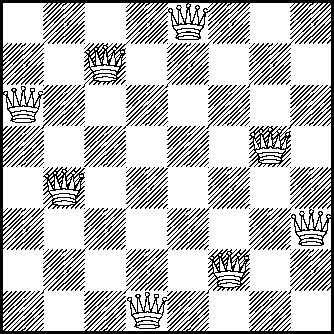
\includegraphics[width=0.35\textwidth]{figuras/8_queens.png}
  \\ Fonte: \cite{apt}
\end{figure}

Para garantir que as rainhas sejam posicionadas de forma a não se atacarem, se faz necessário declarar um conjunto de restrições sobre as variáveis $x_i$. As desigualdades a seguir são suficientes para garantir que os valores de tais variáveis formem uma configuração válida conforme o objetivo do problema, para $i \in [1,n-1]$ e $j \in [i+1,n]$:

\begin{itemize}
  \item $x_i \not= x_j$
  \item $|x_i - x_j| \not= |i - j|$
\end{itemize}

A primeira desigualdade impede que duas ou mais rainhas sejam posicionadas na mesma linha. Tal desigualdade gera um total de $\frac{n(n-1)}{2}$ restrições ao se aplicar todos os possíveis valores de $i$ e $j$. Todas estas restrições juntas garantem que todas as variáveis assumirão valores distintos entre si.

A segunda desigualdade impede que duas ou mais rainhas sejam posicionadas na mesma diagonal. Assim como para a primeira desigualdade, esta também gera um total de $\frac{n(n-1)}{2}$ restrições ao se aplicar todos os possíveis valores de $i$ e $j$, gerando assim um conjunto com $n(n-1)$ restrições ao todo.

Não se faz necessário restrições para verificar se duas ou mais rainhas estão posicionadas na mesma coluna, visto que a forma como o tabuleiro foi modelado já impede naturalmente que tal situação aconteça.



{\bf \textcolor{red}{Faltando .... e melhorar a apresentacao acima}}

\section{Buscas}
{\bf \textcolor{red}{Faltando .... e melhorar a apresentacao acima}}

Referência para esta seção: \cite{rina2003}
UM RESUMO + Taxonomia

\section{Acelerando as Buscas}
{\bf \textcolor{red}{Faltando .... e melhorar a apresentacao acima}}




\section{Conclusões Parciais}
{\bf \textcolor{red}{Faltando .... e melhorar a apresentacao acima}}

\chapter{A Linguagem MiniZinc}


\section{Apresentando o MiniZinc}
\label{sc:minizinc}

Conforme \cite{mzntwds}, antes do advento da linguagem de programação MiniZinc, não existia uma linguagem padrão para a modelagem de problemas de programação por restrições. Praticamente cada \textit{solver} possuia sua própria linguagem de modelagem. Isto dificultava a tarefa de realizar experimentos para comparar o desempenho de diferentes \textit{solvers} para um determinado problema.

O MiniZinc surgiu com a proposta de criar uma linguagem padrão de modelagem, na qual um mesmo modelo pode ser utilizado por diversos \textit{solvers}. 

{\bf \textcolor{red}{Faltando descrever o que sao estes solvers....}}


Além disto, outras de suas qualidades são a simplicidade, a expressividade e a facilidade de implementação \cite{mzntwds}. A simplicidade se encontra principalmente na sintaxe, e a expressividade é dada por permitir modelar diversos tipos de problemas por meio dos recursos disponibilizados.

\section{Elementos da Linguagem}


\subsection{Um Paradigma Computacional}

$$ Modelo + Dados = A_1 \wedge A_2 \wedge A_3 \wedge  ....  \wedge  A_n $$

\begin{itemize}
  \item 
 $A_i: $ são assertivas declaradas (declarações de restrições) sobre o problema

  \item  Logo, esta é uma linguagem  que visa construir rapidamente
modelos sobre os problemas reais.

  \item  Detalhe é que estes \textbf{modelos} são computáveis!


\end{itemize}




\subsection{Estrutura de um Programa em \minizinc}

{\bf \textcolor{red}{Faltando uma figura}}

\subsection{Constantes ou Parâmetros}



As constantes são similares às váriaveis de linguagens de programação comuns. Entretanto, só é permitido atribuir 
um valor a um parâmetro uma vez.

{\bf \textcolor{red}{Faltando ....}}

\subsection{Variáveis}

Variáveis e Variáveis de Decisão (discutidas ao longo do texto) são mais próximas ao conceito de incógnitas da Matemática. O valor de uma váriavel de decisão 
é escolhido pelo Minizinc para atender todas as restrições estabelecidas.


{\bf \textcolor{red}{Faltando ....}}


\begin{description}

  \item[Booleanas:] 
{\bf \textcolor{red}{Faltando ....define e exemplo}}
  
    \item[Inteiras:]
      \item[Reais:]
        \item[Vetores ou Arrays:]
                \item[Conjuntos:]
                
                \item[Enumeradores:]
\end{description}

Contudo, caso estas variáveis exibam um domínio
específico, ou restrito, que é o caso de interesse,
estas variáveis são conhecidas como
\textit{variáveis de restrição}.
Estas assumem valores que   são {\em descobertos} dentro de um domínio 
de valores sob um conjunto de restrições que 
é o  \textit{modelo  computado}.


\subsection{Restrições ou Declarações Lógicas}

{\bf \textcolor{red}{Faltando ....}}
\subsection{Satisfatibilidade e Otimização}

{\bf \textcolor{red}{Faltando ....}}
\subsection{Saídas}

{\bf \textcolor{red}{Faltando ....}}


\subsection{Instalação e Uso}

{\bf \textcolor{red}{Revisao ....}}


\begin{enumerate}   

\item Baixar o arquivo .tar.gz \\\hspace*{0.3cm}(http://www.minizinc.org/g12distrib.html)
\item Extrair a pasta.
\item Executar o arquivo SETUP presente na pasta.
\item Alterar a variável PATH, execute o comando:
\\export PATH=\$PATH:/\textless diretório da pasta do 
minizinc\textgreater/bin
\end{enumerate}





\section{Um Exemplo}

Esta seção apresenta um exemplo completo, o qual  resume os conceitos apresentados anteriormente.
Este exemplo provê noções básicas para compreender e desenvolver programas na linguagem MiniZinc, sendo tais programas comumente chamados de modelos. Para isto, é tomado como exemplo um modelo feito em MiniZinc, apresentado na Figura \ref{code:exemple}.

\lstinputlisting[
    label={code:exemple},
    language=erlang,
    numbers=left, 
    stepnumber=1, 
    frame=single,
    caption={Exemplo de um modelo em MiniZinc}
    ]
    {/home/ccs/Dropbox/CCS/minizinc/nqueens.mzn}


Este é um modelo para o problema das $n$-rainhas, apresentado na Subseção \ref{ss:exemplo-de-modelagem}. A primeira linha contém o comando \textit{include}, que funciona de forma análoga às outras linguagens de programação, como C. Este comando serve para possibilitar a divisão de um mesmo modelo em diversos arquivos e utilizar bibliotecas externas. Neste caso, está sendo incluída a biblioteca de restrições globais por meio do arquivo \textit{globals.mzn}, com o intuito de utilizar a restrição \textit{alldifferent}, pertencente a tal biblioteca, no modelo.

Na linha 3 está sendo declarada a variável $n$ e atribuindo a esta o valor $8$. Tal variável representa o tamanho do tabuleiro, e por consequência a quantidade de rainhas presentes neste. Na linguagem MiniZinc as variáveis podem ser parâmetros ou variáveis de decisão. Os parâmetros são variáveis de valor fixo e conhecido. Já as variáveis de decisão são variáveis cujo valor será atribuído pelo \textit{solver}, de forma a satisfazer todas as restrições.

Os valores dos parâmetros podem ser definidos tanto no próprio modelo, como no caso do modelo apresentado na Figura \ref{code:nqueens}, ou em um arquivo externo de extensão \textit{.dzn}. Caso o usuário esteja utilizando a IDE do MiniZinc, também é possível fornecer os valores dos parâmetros por meio de uma interface gráfica. Tal interface é exibida ao usuário quando este pressiona o botão para executar o modelo e os valores dos parâmetros não são fornecidos no código.

Ao se declarar uma variável em MiniZinc, se faz preciso informar o tipo desta e se esta é um parâmetro ou uma variável de decisão. Entre os tipos de variável disponíveis estão, por exemplo, \textit{int}, \textit{float} e \textit{bool}.

Para se especificar que uma váriavel é de decisão, é necessário utilizar o prefixo \textit{var} antes do tipo da variável. Caso não haja um prefixo antes do tipo de uma variável, o MiniZinc irá considerar esta como sendo um parâmetro, apesar de ser possível utilizar o prefixo \textit{par} para se explicitar que esta é um parâmetro. Desta forma, a variável $n$ declarada na linha 3 é um parâmetro, visto que não há o prefixo \textit{var} antes desta.

Na linha 4 há a declaração do vetor \textit{pos\_rainhas}, que neste modelo representa as posições das rainhas. Neste vetor, a i-ésima posição representa a linha na qual se encontra a rainha que está na i-ésima coluna do tabuleiro.
  
Para se declarar um vetor em MiniZinc, se faz necessário definir o intervalo de índices de cada uma de suas dimensões, o tipo dos seus elementos e se estes são parâmetros ou variáveis de decisão.

No caso do vetor \textit{pos\_rainhas}, há apenas uma dimensão, sendo que os índices variam de $1$ até o valor do parâmetro $n$. Os índices possíveis de cada uma das dimensões do vetor são especificados dentro dos colchetes, após a palavra chave \textit{array}.

Os elementos do vetor \textit{pos\_rainhas} são variáveis de decisão, visto que o intuito do modelo é justamente encontrar as posições em que as rainhas devem ser posicionadas. Neste caso, os valores que os elementos podem assumir estão restringidos a um domínio finito, que é o intervalo inteiro que varia de $1$ até $n$.

A linha 6 apresenta a primeira restrição do modelo, que garante que o valor do parâmetro $n$ informado pelo usuário é maior que três. As restrições em MiniZinc devem iniciar com a palavra chave \textit{constraint} e devem ser expressões booleanas, isto é, devem resultar em verdadeiro ou falso. Tais expressões podem envolver parâmetros, variáveis de decisão e constantes, que devem ser relacionados por meio de algum operador de relação, como $>$, $<=$, $=$ e $!=$.

Para facilitar a modularização dos modelos, o MiniZinc possibilita a definição de predicados, e a partir da versão 2.0, também permite a definição de funções. A linha 8 mostra o predicado \textit{alldifferent}, que faz parte da biblioteca de restrições globais do MiniZinc. Este predicado recebe um vetor de inteiros e garante que os valores dos elementos deste vetor são distintos entre si. Esta restrição é equivalente à primeira desigualdade apresentada na Subseção \ref{ss:exemplo-de-modelagem}.

Na linha 10 é apresentada uma restrição um pouco mais complexa. Esta faz uso do \textit{forall}, que funciona de forma análoga ao quantificador universal $\forall$. Em MiniZinc, utiliza-se o \textit{forall} principalmente quando deseja-se agrupar diversas restrições semelhantes, de modo a simplificar a leitura e o desenvolvimento do modelo. Normalmente tais restrições semelhantes estão vinculadas a vetores ou conjuntos, e se faz possível generalizar estas restrições utilizando iteradores.

Uma das formas de se utilizar o \textit{forall} é especificando um iterador, o conjunto de possíveis valores que este pode assumir e a restrição generalizada em termos deste iterador. Desta forma, para cada um dos valores que o iterador pode assumir será gerada uma expressão \textit{booleana}, em que o iterador será substituido pelo valor assumido. Todas estas expressões geradas são unidas em uma única restrição, sendo que tal união é feita por meio da conjunção de todas as expressões. Desta forma, para que a restrição criada seja satisfeita, todas as expressões \textit{booleanas} geradas devem resultar em verdadeiro.

A linguagem MiniZinc também oferece o \textit{exists}, que funciona de forma praticamente igual ao \textit{forall}, sendo que a única diferença entre estes está na forma como as expressões \textit{booleanas} são unidas, que neste caso é por meio de disjunções. Assim, para que a restrição criada pelo \textit{exists} seja satisfeita, basta que uma das expressões que compõem a restrição seja satisfeita.

No caso da restrição presente na linha 10, o \textit{forall} é utilizado duas vezes, de forma aninhada. Isto é feito pois se faz necessário garantir que todos os pares possíveis de rainhas não estão se atacando mutuamente.

A linha 12 apresenta a expressão \textit{booleana} que verifica se um par de rainhas está ou não se atacando, de forma equivalente à segunda desigualdade apresentada na Seção \ref{ss:exemplo-de-modelagem}. A função \textit{abs} retorna o valor absoluto, ou o módulo, de um inteiro.

Na linha 16, há a indicação de que o problema é de satisfação de restrições. Caso fosse um problema de otimização, seria necessário substituir a palavra chave \textit{satisfy} por \textit{maximize} ou \textit{minimize}, seguido da função que se deseja maximizar ou minimizar.

Por fim, na linha 18 há o comando \textit{output}, pelo qual pode-se imprimir na tela os resultados obtidos. Tal comando é bastante flexível, de forma que saídas complexas podem também ser geradas. Para este problema seria possível, por exemplo, imprimir o tabuleiro utilizando algum caracter para representar as rainhas.

Na biblioteca apresentada no capítulo 4, as funcionalidades são implementadas por meio de funções. Isto é feito para que seja possível utilizar esta biblioteca em qualquer modelo, bastando para isto incluir um arquivo, como foi feito neste exemplo para utilizar a biblioteca de restrições globais. Para exemplificar a definição de funções, a Figura \ref{code:nqueens} apresenta um modelo equivalente ao apresentado anteriormente, entretanto, utilizando uma função para a resolução do problema.

\lstinputlisting[
    label={code:nqueens},
    language=erlang,
    numbers=left, 
    stepnumber=1, 
    frame=single,
    caption={Exemplo de utilização de função}
    ]{/home/ccs/Dropbox/CCS/minizinc/nqueens_fn.mzn}


Na linha 6 deste exemplo, há a declaração da função. Esta é iniciada com a palavra chave \textit{function}, que é sucedida pela declaração do tipo de retorno da função. Em MiniZinc, toda função precisa obrigatoriamente de um retorno, visto que quando este não se faz necessário pode-se substituir o uso de uma função pelo uso de um predicado.

Após o tipo de retorno, há o identificador da função, que é utilizado na hora de realizar chamadas à função. Após o identificador, há a lista de argumentos da função. Para cada argumento é especificado um tipo e um identificador.

Neste exemplo, a função é chamada de \textit{n\_queens} e recebe como argumento o tamanho do tabuleiro desejado, identificado como \textit{num\_of\_queens}. O retorno desta função é um vetor no qual os elementos são variáveis de decisão inteiras. Este vetor representa uma possível solução para o problema, de acordo com a modelagem proposta anteriormente.

A estrutura \textit{let\{\} in} presente na função, permite o uso de variáveis locais. De forma geral, quando esta estrutura é utilizada em funções, pode-se comparar o conteúdo presente dentro do \textit{let} como sendo o corpo da função, e a expressão após o \textit{in} como sendo o retorno desta.

Após a conclusão de um modelo, se faz preciso utilizar um \textit{solver} para encontrar os valores das variáveis de decisão, de forma a satisfazer todas as restrições. Isto pode ser feito, por exemplo, pela própria IDE fornecida pelo MiniZinc, na qual pode-se editar os modelos e avaliá-los. Caso não haja uma solução possível, o MiniZinc apresenta uma mensagem informando que o modelo é insatisfatível, ou seja, não existe uma atribuição de valores às variáveis de decisão que satisfaça as restrições estabelecidas. Há ainda casos em que o modelo em questão pode ter muitas possibilidades de soluções para serem avaliadas, gerando uma explosão combinatorial, o que pode fazer com que o \textit{solver} não consiga encontrar uma solução em um tempo aceitável.

Para a implementação da biblioteca, alguns outros recursos do MiniZinc que não são explicados nesta seção são utilizados. Porém, tais recursos são explicados à medida em que são utilizados nas implementações.




\section{Conclusões Parciais}
{\bf \textcolor{red}{Faltando .... e melhorar a apresentacao acima}}


\chapter{Modelagem de Problemas}
\label{cp:mp}


Neste capítulo são apresentados alguns estudos de casos.

\section{Os Modelos em Estudo}

XXXXXXXXXXXXXXXXXXXXX ... bons modelos e classicos  interessantes ....

%%
\section{Cripto-Aritméticos}

\subsection{O que é um cripto-aritmético?}

A common puzzle is to present a math problem where each digit is replaced by a letter.  So, for example the sum:
\begin{verbatim}
   112
+  234
---------
   346
could be represented as:
  AAB
+ BCD
---------
  CDE
\end{verbatim}
where $A=1$, $B=2$, $C=3$, $D=4$, and $E=6$.  Notice that the same digit always replaces all instances of the same letter.  It will also be the case that each distinct letter will be replaced by a different digit.

Estes problemas são importantes para PR pois ilustram .......... falta escrever 


\subsection{Alguns Criptos}

Sua tarefa é resolver os seguintes criptos-aritméticos para o domínio
$0$ a $9$ de todas variáveis mencionadas nas
proposições.

\begin{description}
\item [ONE + ONE = TWO]

  \item[BASE + BALL = GAMES] 

\item [WRONG + WRONG = RIGHT]

%%%[O,N,E], [O,N,E], [T,W,O]).
\end{description}


\subsection{A Equação \/ ``{\em Mágica}''}

 Seja a equação \/ ``{\em mágica}''\/ dada por:
$$
\frac{A}{B \times C} + \frac{D}{E \times F} + \frac{G}{H \times I} = 1
\label{eq_fracao}
$$
Elabore um programa que encontre valores distintos para as $9$ variáveis
da equação \ref{eq_fracao}, no domínio de $1$ a $9$, tal que
os valores sejam todos distintos.\\

Que outra(s) estratégia voce resolveria este problema?



\section{Ilustrando a PR}

%%{\bf \textcolor{red}{Vou refazer novos desenhos... aguardem}}

 O objetivo destes problemas é ilustrar o paradigma da PR.
Para cada uma das ilustrações que se seguem,
construa um programa que retorne o número de pontos válidos na implementação 
de seu modelo. O domínio da variável $x$ e $y$ são inteiros,
e tem seus limites dado pelas figuras.

Faça as suposições que julgares necessárias, visando as melhorias
deste problema e seu objetivo (acompanhe as aulas). Seu primordial
objetivo é ilustrar a PR via várias áreas do Espaço de Estados (EE) 
de um problema.



\subsection{O brasão da CroáXia}

 A CroáXia é um belo país, e tem uma bandeira
  um pouco bizarra, mas a parte marcante é são as cores do seu brasão, representando
  as duas etnias predominantes deste país. Assim, como todo aluno
  da CroáXia deve conhecer o brasão, lá eles usam o mesmo para ensinar matemática.
  Há bons matemáticos por lá, mas pediram ajuda para saber quais os pontos 
  na amostra abaixo e qual a área em vermelho.

 \begin{figure}[!ht]
  \centering
    %\reflectbox{%
      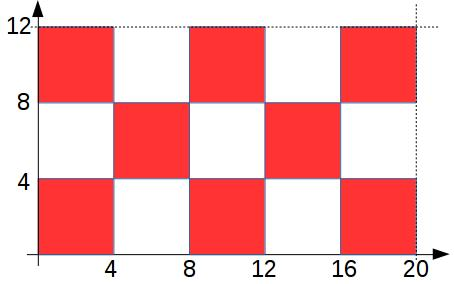
\includegraphics[width=0.5\textwidth , height=0.25\textheight]{croacia_flag.jpg}
      %%}
      \caption{Ilustrando a PR}
\label{fig_croacia}
\end{figure}

As áreas hachuradas da figura \ref{fig_croacia} são pontos válidos da solução,
logo, extremidades são contabilizadas como soluções válidas. Outro detalhe,
que algumas destas restrições, são fornecidas por funções tais como, por 
exemplo: $| x - y| \:\: mod \:\:  4$, logo, use-a.
O número de pontos ou soluções válidas
no Minizinc, são obtidas ao se habilitar as opções de \textit{verbose solving} 
e \textit{statitics for solving}, pois cada ponto válido é uma soluçao para este problema.



\subsection{Quais são os pontos no triângulo?}

Quais são os pontos da área definida pelo triângulo da figura \ref{fig_triangulo}?

 \begin{figure}[!ht]
  \centering
    %\reflectbox{%
      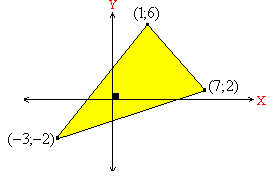
\includegraphics[width=0.5\textwidth , height=0.2\textheight]{triangulo_amarelo.png}
      %%}
      \caption{Ilustrando a PR}
\label{fig_triangulo}
\end{figure}
Basta imprimir os pontos válidos dentro desta área. O número de pontos ou soluções válidas
no Minizinc, são obtidas ao se habilitar as opções de \textit{verbose solving} e \textit{statitics for solving}, pois cada ponto válido é uma soluçao para este problema.





\subsection{Quais são os pontos? -- 01}
 Quais são os pontos definidos  pela área  da figura \ref{fig_area_validas01}?
 \begin{figure}[!h]
  \centering
    %\reflectbox{%
      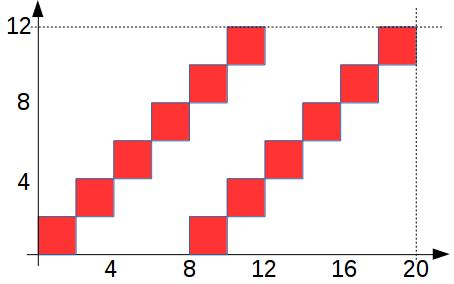
\includegraphics[width=0.5\textwidth , height=0.25\textheight]{area_validas01.jpg}
      %%}
      \caption{Ilustrando a PR}
\label{fig_area_validas01}
\end{figure}

Basta imprimir os pontos válidos dentro desta área. O número de pontos ou soluções válidas
no Minizinc, são obtidas ao se habilitar as opções de \textit{verbose solving} e \textit{statitics for solving}, pois cada ponto válido é uma soluçao para este problema.



\subsection{Quais são os pontos? -- 02}

 Quais são os pontos definidos  pela área da figura \ref{fig_area_validas02}?
 \begin{figure}[!ht]
  \centering
    %\reflectbox{%
      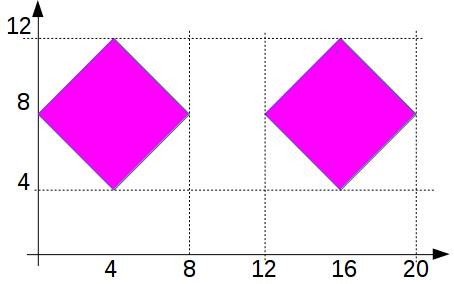
\includegraphics[width=0.5\textwidth , height=0.25\textheight]{area_validas02.jpg}
      %%}
      \caption{Ilustrando a PR}
\label{fig_area_validas02}
\end{figure}

Basta imprimir os pontos válidos dentro desta área. O número de pontos ou soluções válidas
no Minizinc, são obtidas ao se habilitar as opções de \textit{verbose solving} e \textit{statitics for solving}, pois cada ponto válido é uma soluçao para este problema.



\subsection{Quais são os pontos? -- 03}

Quais são os pontos definidos  pela área hachurada da figura \ref{fig_area_validas03}?
 \begin{figure}[!hb]
  \centering
    %\reflectbox{%
      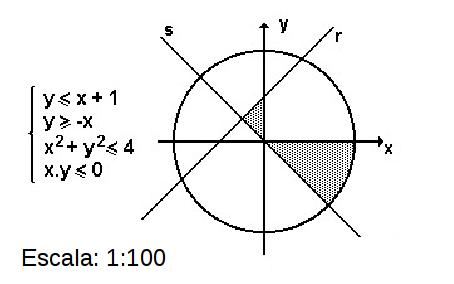
\includegraphics[width=0.5\textwidth , height=0.2\textheight]{area_validas03.jpg}
      %%}
      \caption{Refazer esta figura bem como as equações-- Escala 1:100 $x$ 100}
\label{fig_area_validas03}
\end{figure}


Basta imprimir os pontos válidos dentro desta área. O número de pontos ou soluções válidas
no Minizinc, são obtidas ao se habilitar as opções de \textit{verbose solving} e \textit{statitics for solving}, pois cada ponto válido é uma soluçao para este problema.



\section{Cripto-Aritméticos}

\subsection{O que é um cripto-aritmético?}

A common puzzle is to present a math problem where each digit is replaced by a letter.  So, for example the sum:
\begin{verbatim}
   112
+  234
---------
   346
could be represented as:
  AAB
+ BCD
---------
  CDE
\end{verbatim}
where $A=1$, $B=2$, $C=3$, $D=4$, and $E=6$.  Notice that the same digit always replaces all instances of the same letter.  It will also be the case that each distinct letter will be replaced by a different digit.

Estes problemas são importantes para PR pois ilustram .......... falta escrever 


\subsection{Alguns Criptos}

Sua tarefa é resolver os seguintes criptos-aritméticos para o domínio
$0$ a $9$ de todas variáveis mencionadas nas
proposições.

\begin{description}
\item [ONE + ONE = TWO]

  \item[BASE + BALL = GAMES] 

\item [WRONG + WRONG = RIGHT]

%%%[O,N,E], [O,N,E], [T,W,O]).
\end{description}


\subsection{A Equação \/ ``{\em Mágica}''}

 Seja a equação \/ ``{\em mágica}''\/ dada por:
$$
\frac{A}{B \times C} + \frac{D}{E \times F} + \frac{G}{H \times I} = 1
\label{eq_fracao}
$$
Elabore um programa que encontre valores distintos para as $9$ variáveis
da equação \ref{eq_fracao}, no domínio de $1$ a $9$, tal que
os valores sejam todos distintos.\\

Que outra(s) estratégia voce resolveria este problema?


\section{Cabo de Guerra}

%%%%%%%%%%%%%%%%%%%%%%%%%%%%%%%%%%%%%%%%%%%%%%%%%%%%%%%%%%%%%
\subsection{Descrição}

\textcolor{red}{Melhorar o enunciado ... mas o outros estão melhores}\\

Várias crianças se encontram para 
 brincadeira do cabo-de-guerra no pátio da escola. Como será
 feita a divisão entre as  duas equipes?   ``{\em Por peso}''\/ grita o mais eufórico. Que seja feita a divisão dos times  sobre uma sequência/lista de peso tal como:
 
\begin{center}
\begin{tabular}{|c|c|c|c|c|}
\hline
$Joao_1$ & $Pedro_2$ & $Manoel_3$ & .... & $Zeca_n$ \\ \hline
45 & 39 & 79 & .... & 42  \\ \hline
\end{tabular}
\end{center}

\ding{224} Preencha a tabela acima com inteiros e valores de sua família.

\ding{224}  Sim, por peso, todos concordaram,
 ``{\em exceto que a divisão deveria respeitar o critério $|N_A - N_B| \le 1$}'', disse o 
mais cauteloso. Sim, nenhum time poderia duas crianças a mais que ou outro time. 

%%%%%%%%%%%%%%%%%%%%%%%%%%%%%%%%%%%%%%%%%%%%%%%%%%%
\subsection{Especificação}

Que seja feita a divisão:

 
\begin{center}
\begin{tabular}{|c|c|c|c|c|}
\hline
$Joao_1$ & $Pedro_2$ & $Manoel_3$ & .... & $Zeca_n$ \\ \hline
45 & 39 & 79 & .... & 42  \\ \hline
\end{tabular}
\end{center}

\begin{itemize}
\item Divisão  por peso
\item Respeitar  critérios como: $|N_A - N_B| \le 1$
\item Todos devem brincar

\item \textsf{Bem, esta simples {\bf \underline{restrição}} ({\bf $|N_A - N_B| \le 1$}), de nosso cotidiano tornou um simples problema em mais uma questão combinatória.
 Um arranjo da ordem de  $\frac{n!}{(n/2)!}$.
 Casualmente, nada trivial  para grandes valores! }
 \end{itemize}


\ding{224} Dois detalhes:

\begin{enumerate}
\item Na tabela de pesos, use valores {\bf inteiros};

\item Use os pesos de seus familiares para completar esta tabela
com um quantidade significativa;

\item No lugar de {\em array} como estrutura base, use {\em sets} para armazenar
e manipular estes valores. Com certeza ficará mais  {\em elegante}, e 
possivelmente mais ineficiente. Teste e comprove!

\end{enumerate}

%%%%%%%%%%%%%%%%%%%%%%%%%%%%%%%%%%%%%%%%%%%%%%%%

\subsection{Modelagem}

 \begin{itemize}

  \item Usando uma variável de decisão: análogo a árvore do SAT  
 
\begin{center}
\begin{tabular}{|l|c|c|c|c|c|}
\hline
Nomes ($n_i$): & $n_1$ & $n_2$ & $n_3$ & .... & $n_n$ \\ \hline
Peso ($p_i$): & 45 & 39 & 79 & .... & 42  \\ \hline
Binária ($x_i$): & 0/1 & 0/1 & 0/1 & .... & 0/1  \\ \hline
\end{tabular}
\end{center}
  
\item Assim $N_A \approx N/2$, $N_B \approx N/2$  e  $|N_A - N_B| \le 1$   

\item $x_i = 0$: $n_i$ fica para o time $A$
\item $x_i = 1$: $n_i$ fica para o time $B$
\item Logo a soma:
$$\sum_{i=1}^n x_i p_i$$ é o peso total do time $B$ ($P_B$)
  
  \end{itemize}

%%%%%%%%%%%%%%%%%%%%%%%%%%%%%%%%%%%%%%%%%%%%%%%%%

  \begin{itemize}
  \item Falta encontrar peso total do time $A$ ($P_A$), dado por: 

  \item $P_A = P_{total} - P_B$
  
  \item  ou $$P_A = \sum_{i=1}^n p_i - \sum_{i=1}^n x_i p_i$$   

  \item Finalmente, aplicar uma minimização  na diferença: $|P_A - P_B|$
  
%%  \item A seguir, tudo isto em código:
  
  \end{itemize}

%%%%%%%%%%%%%%%%%%%%%%%%%%%%%%%%%%%%%%%%%%%%%%%%%
\subsection{Estratégia}%%% de Implementação}

Uma árvore de decisão binária ............ descreva como
voce implementou ou a fundamentacao

\begin{figure}[ht!]
 \centering
 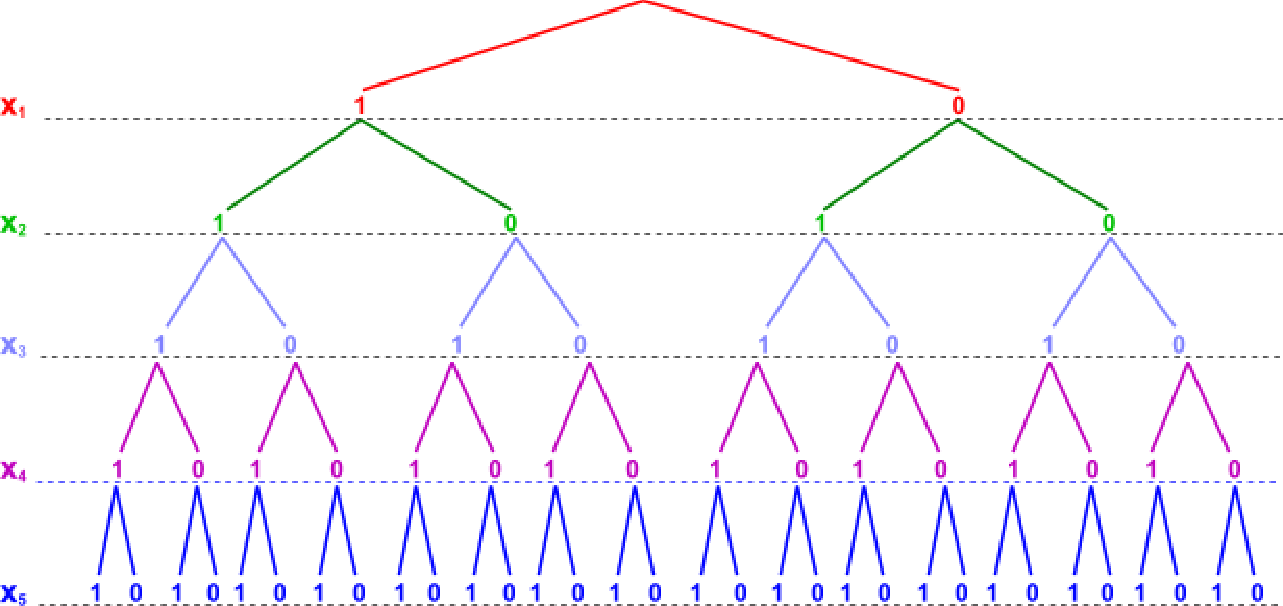
\includegraphics[width=0.7\textwidth , height=0.3\textheight]{binary_tree04.pdf}
\caption{Se $x_i=0$, então $n_i$ segue para o time $A$, caso  $x_i=1$, então  $n_i$ vai para o time $B$} 
%\label{}
\end{figure}

%%%%%%%%%%%%%%%%%%%%%%%%%%%%%%%%%%%%%%%%%%%%%%%%%
\subsection{Implementação}

O código fonte se encontra em:

\url{https://github.com/claudiosa/CCS/tree/master/minizinc/cabo_de_guerra.mzn}

%%%%%%%%%%%%%%%%%%%%%%%%%%%%%%%%%%%%%%%%%%%%%%%%%
\subsection{Resultados e Análise}


Considerando pesos aleatórios de 1 a 150 para as pessoas

Usando um \textit{solver} médio do Minizinc (\textit{G12 lazyfd}) padrão:

\begin{table}
  \caption{Resultados ...................}
   \label{tab:}
  
  \begin{center}
  \begin{tabular}{ l | c |c | r }
    \hline  \hline 
    $n$ & tempo & $P_A$ & $P_B$\\ \hline     \hline 
     5 & 40msec & 276 & 278 \\ \hline
    10 & 46msec & 518 & 519 \\ \hline
    25 & 98msec & 1198 & 1197 \\ \hline
    50 & 411msec & 2290 & 2291 \\ \hline
    75 & \textbf{\textcolor{red}{2s 485msec}} & 3133 & 3133 \\ \hline
    100 & 470msec & 4142 & 4142 \\ \hline 
    125 & \textbf{\textcolor{red}{7s 2msec}} & 4992 & 4992 \\ \hline 
    150 & 605msec & 5823 & 5823 \\ \hline 
    175 & 642msec &   6777 &  6778 \\ \hline 
    200 & $>$ 10min & -- & -- \\ \hline \hline
  \end{tabular}
  
\end{center}

\end{table}
Referência: cpu 4-core, 4 G ram, SO: Linux-Debian

%%%%%%%%%%%%%%%%%%%%%%%%%%%%%%%%%%%%%%%%%%%%%%%%%%%%%%%%%%%%%%%%%%%%%%%%%%%%%%%%%%%%%%%%%%%%%%%%%%%%%%%%%%%%%%

%%\input{capitulo-4_MODELOS/proximos_modelos/modelos.tex}
%%\input{capitulo-4_MODELOS/proximos_modelos/modelos.tex}
%%\input{capitulo-4_MODELOS/proximos_modelos/modelos.tex}

%\input{cap1/cap1.tex}
%\input{cap2/cap2.tex}
%\input{cap3/cap3.tex}
%\input{cap4/cap4.tex}


\appendix

\bibliographystyle{plain}
\bibliography{refs_CP}

\end{document}
